\documentclass[11pt]{article} % do not change this line
\input{BigDataStyle.txt}      % do not change this line
\usepackage{algorithm,algpseudocode,amsfonts,amssymb,amsthm,amsmath,graphicx,hyperref,latexsym,nicefrac,subcaption,titlesec}

\emergencystretch=5mm
\tolerance=400
\allowdisplaybreaks[4]

\theoremstyle{plain}
\newtheorem{theorem}{Theorem}[section]
\newtheorem{proposition}[theorem]{Proposition}
\newtheorem{corollary}[theorem]{Corollary}
\newtheorem{lemma}[theorem]{Lemma}
\newtheorem{problem}[theorem]{Problem}

\theoremstyle{definition}
\newtheorem*{remark}{Remark}

\title{Aggregating Algorithm}
\author{Candidate 2408208}

\newcommand{\Programme}{Machine Learning}
% Computational Finance students: uncomment the next line
%\twodepartmentstrue

\newcounter{protocol}
\makeatletter
\newenvironment{protocol}[1][htb]{
  \let\c@algorithm\c@protocol{}
  \renewcommand{\ALG@name}{Protocol}
  \begin{algorithm}[#1]
  }{\end{algorithm}
}
\makeatother

\setcounter{secnumdepth}{4}
\titleformat{\paragraph}
{\normalfont\small\bfseries}{\theparagraph}{1em}{}
\titlespacing*{\paragraph}
{0pt}{3.25ex plus 1ex minus .2ex}{1.5ex plus .2ex}

\titleformat{\subparagraph}
{\normalfont\footnotesize\itshape}{\theparagraph}{1em}{}
\titlespacing*{\subparagraph}
{0pt}{3.25ex plus 1ex minus .2ex}{1.5ex plus .2ex}

\begin{document}
\maketitle

\declaration{}

\begin{abstract}
  Your abstract goes here.

  \textbf{Keywords:} On-line Learning, Prediction with Expert Advice, Aggregating Algorithm for Specialist Experts, Perceived Randomness
\end{abstract}

\section*{Acknowledgements}
While the contents of this report are based on my work, none of this would have been possible without the patience and mentorship of my supervisor to whom I am extremely grateful. It was your advice, clear explanations, and expertise that made this project what it is now and something that I am incredibly proud of.
I would also like to express my gratitude to the group of friends who made this academic year possible, namely Cougar Tasker, Einstein Ebereonwu, Hayden Amarr, Mohammadreza Yazdian, Niraj Jain, and Ray Mahbub, without whom I would have struggled to maintain my discipline and motivation.
\newpage

\section{Introduction}\label{section:introduction}

\subsection{Project Scope and Objectives}
The aim of this project is to implement the Aggregating Algorithm for Specialist \textit{(Sleeping)} Experts, a method of Prediction with Expert Advice, to scenarios involving human-generated sequences and evaluate its predictive performance in pre-empting what the human subject will input, effectively testing how good human subjects are at generating random inputs.

As an introduction to the concepts that will be explored in the sections to come, this algorithm allows for the effective pooling of different prediction algorithms, known as `Experts', in order to improve the algorithm's prediction accuracy. By aggregating several predictions, this allows the final prediction outputted by the algorithm to be nearly as accurate as the best-performing Expert.

This project will encompass several key areas, including:
\begin{itemize}
    \item \textbf{Explaining the Theory of Perceived Randomness.} The basis of this study revolves around the human perception of randomness, which is different to objective randomness, therefore the underlying psychological mechanisms for how humans judge and perceive randomness must be understood.
    \item \textbf{Explaining the Theory of Prediction with Expert Advice.} The other portion of this study is firmly based in the subject matter of Prediction with Expert Advice, primarily focussing on the Aggregating Algorithm and the Aggregating Algorithm for Speciallist Experts so the underlying theory must be explored with a thorough review of the current literature.
    \item \textbf{Implementing the Aggregating Algorithm.} This project will primarily investigate the Aggregating Algorithm introduced by Vovk (see~\cite{vovk:1990},\ \cite{vovk:1998}).
    \item \textbf{Handling Specialist Experts.} Introduced by Freund~\cite{freund:1997}, \textit{Specialist Experts} may refrain from making predictions at certain points, meaning that the Aggregating Algorithm has to be modified slightly~\cite{kalnishkan:2015}.
    \item \textbf{Evaluating the Performance of Human Subjects in Generating Statistically Random Seuqences.} Through conducting the experiment outlined in this paper, this study will present how well the subjects were able to generate a ``random'' sequence when compared to the statistical definition used by statisticians.
    \item \textbf{Evaluating the Performance of the Algorithm in Predicting Human-Generated Outcomes.} The experiment will also compare how well the Aggregating Algorithm for Specialist Experts was able to pre-empt each subject's sequences, in a somewhat adversarial comparison to statistical randomness.
\end{itemize}

\subsection{Motivation and Interest in the Subject Area}
The motivation for selecting a project in this subject area is rooted in both my personal and professional interests, as well as the discussions I had with my now-supervisor, Dr.\ Yuri Kalnishkan, before finalising my selection.

During this academic year, the module that most piqued my interest was CS5200 \textendash\ On-line Machine Learning because I was interested in the techniques that allowed machine learning models to gradually improve over time as more data became available to them without the need to retrain the model on the entire newly-updated dataset; something that had not been covered previously by other modules. Due to the module's small size and frequent absentees, I was able to gain a deeper understanding of the module, in large part due to Dr.\ Kalnishkan's willingness to explain portions of the syllabus in extreme detail. Alongside the lectures, I felt like I was strongly suited to the contents of the module because it has strong ties to the field of statistics \textendash\ another area that I thoroughly enjoyed throughout my education.

Regarding my professional aspirations, I am set to begin my career later this year and I am of the firm belief that the work that I have done in this subject area is highly relevant, not only to the job I am to start in September, but also for my career plan due to its relevance across a variety of industries \textendash\ including finance, energy, and insurance.

Ultimately, the combination of all of these factors led me to pursue a project investigating on-line prediction, and prediction with expert advice.

\subsection{Structure of the Dissertation}
The following study is split into several distinct chapters and subsections, each dedicated to exploring a specific aspect behind the study being conducted. The following outline guides you, the reader, through the report by providing a brief overview of the contents of each chapter.

Chapter~\ref{section:literature_review} contains the Literature Review that is organised to explain the underlying theory that the practical portion of this study aims to investigate.

Section~\ref{subsection:perceived_randomness} explores the human perception of randomness and how it is, in fact, different from the objective definition of randomness, and aims to provide context to answer the question ``Are humans good randomisers?'' in both judgement and generation scenarios.

Section~\ref{subsection:prediction_with_expert_advice} is diverse in its contents. Subsection~\ref{subsubsection:introduction_to_on-line_prediction} defines the problem of On-line Prediction, outlining the scenarios in which it is applicable, and the protocols that such problems follow. Additionally, it explores how On-line Prediction differs from the traditional Machine Learning frameworks of Batch Learning and Timeseries Analysis and defines concepts that will be critical to understanding the experiment being conducted. Subsection~\ref{subsubsection:prediction_with_expert_advice} expands on the information presented in the previous subsection by defining the modifications to the original framework to now incorporate the predictions made by a pool of Experts and how the Learner aggregates those to inform its own. It also gives two examples of merging strategies that could be used to accomplish that task. Subsection~\ref{subsubsection:aggregating_algorithm} introduces the algorithm that is the main focus of this study, delving into the rationale behind the algorithm and discussing the bounds guaranteed by utilising it. Lastly, Subsection~\ref{subsubsection:aggregating_algorithm_for_specialist_experts} defines a modification to the original Aggregating Algorithm that allows it to be used in scenarios involving Specialist Experts, a term used to define any Expert that has the ability to abstain from making a prediction.

Chapter~\ref{section:experiment_design_and_methodology} is centred on the practical applications of the theory and how it was used to derive the experiment that is to be conducted, including how the experiment was designed, how the Aggregating Algorithm was applied to the proposed scenario and how the data gathered from the subjects will be analysed.

Chapter~\ref{section:analysis_of_perceived_randomness} will discuss the findings of the study in detail, ultimately attempting to answer the hypothesied question ``are humans good randomisers?''.

Finally, Chapter~\ref{section:conclusion} contains a conclusion that summarises the findings of the study, as well as a self-evaluation of the project.

\newpage

\section{Literature Review}\label{section:Literature_Review}
\subsection{Introduction}
\textbf{Purpose:} Overview of the goals of the literature review.\newline
\textbf{Scope:} Outline of the topics covered and their relevance to the dissertation.\newline
\noindent\rule{\textwidth}{0.1pt}
\subsection{Perceived Randomness}
\subsubsection{Are Humans Good Randomisers?}
The definition of the term ``random'' is a contentious area for debate. In essence, randomness is an unobservable characteristic of a generating process therefore the act of trying to define it is somewhat contradictory. In order to determine if a process or sequence is random, it has to be put through statistical tests for specific properties which are deemed to be ``random''. However, because these tests are statistical in nature, are the conclusions drawn objectively random or purely subjective?

Research into the human perception and generation of random sequences is a common topic within psychological papers, yet the contradictory nature of findings results in a less-than-satisfactory answer to the question of ``Are humans good randomisers?'' (much like when defining the term itself).

The origins of such a question can be traced back to an observation made by Hans Reichenbach in The Theory of Probability, 1949~\cite{reichenbach:1949}; he suggested that when asked to produce a series that seemed random to them, people untrained in the theory of probability would be unable to generate such a series and, instead, generate one that would contain patterns and biases, e.g.\ too many alternations than what was expected. This ultimately suggests that humans are not good randomisers which is the prevalent opinion to date. This behaviour is attributed to the fact that human-generated sequences often reflect the underlying psychological tendencies of subjects, rather than the unpredictability of true randomness.

While Reichenbach assumes the stance that humans are not good randomisers, the alternative to this conclusion was put forward by the work of Bruce Ross~\cite{ross:1955}. Ross explores the processes involved in randomising binary sequences and analyses the methods that people used, as well as the typical mistakes that they made, when attempting to create random sequences. In his study, Ross got 60 subjects to stamp cards with either an `$\mathcal{O}$' or an `$\mathcal{X}$' and  place them singly in a $100$-item sequence in the middle of a table that they thought to be random, with item frequencies of either $50-50$, $60-40$, or $70-30$. These sequences were then scored against the expected properties of a random sequence and, based on the analysis conducted, resulting in the conclusion that ``the prevalent \textit{a priori} assumption that the human being is a systematically biased randomi[s]er was not borne out.''~\cite{ross:1955}

\subsubsection{Judgement vs. Production of Random Binary Sequences}
As alluded to by the question posed in the previous subsection, the human perception of randomness is a subjective, rather than objective, quality. Because of this subjectivity, two natural interpretations can follow—either that subjects have an incorrect idea of what randomness is and should look like, or that subjects intuitively know what true randomness should look like but some internal functional limitation prevents the judgement and production of such sequences~cite{wagenaar:1970}, being so powerful that subjects may choose to forego statistical analysis in favour of this intuitive ``gut feeling''~cite{bar-hillel:1991}. Since the main topic of this dissertation is Prediction with Expert Advice (to be introduced in the following subsection) for $\eta$-mixable games, the focus of this literature review will be on the judgement and production of random binary sequences. Both types of study make interesting observations about the internal mechanism responsible for the human perception of randomness, namely ``that [humans] see clumps or streaks in truly random series and expect more alternation, or shorter runs, than are there'' and ``[humans] produce series with higher than expected alternation rates''~\cite{bar-hillel:1991}.

We will first explore judgement. In Willem Wagenaar's 1970 study titled ``Appreciation of conditional probabilities in binary sequences'', he examines people's comprehension of conditional probabilities, focusing on how people perceive and interpret the likelihood of certain events occurring given previous outcomes~\cite{wagenaar:1970}. Through conducting this experiment, this research reveals a significant gap in understanding and the systematic biases that affect our judgements of conditional probabilities.

The study controlled the conditional probability of a $0$ after $0$ ($1$ after $1$) as the experimental variable, testing it in the range $0.2-0.8$ with $0.1$ increments, i.e. 7 values of conditional probability, for first-, second-, and third-orders of dependency. Participants were then shown 16 sets of 7 binary sequences (generated with one of these values of conditional probabilities) for each order of dependency and asked to select and record the sequence that looked the most random to them—explained as the sequence that looked the most likely to be produced when flipping a fair coin. For reference, in a truly random binary sequence, the conditional probability of $0$ after $0$ ($\text{Pr}(0|0)$) or $1$ after $1$ ($\text{Pr}(1|1)$) for the first order of dependency is $0.5$. However, Wagenaar identified that conditional probabilities close to $0.4$ were perceived as the most random across all orders of dependencies, affirming the position that humans aren't good randomisers and that there is some subjective concept of randomness. This study also highlights the bias in favour of `negative recency', more commonly known as the gambler's fallacy wherein gamblers will tend to bet on red after a run of blacks (and vice versa) on a roulette wheel, ultimately causing humans to favour series with slightly more alternations than is expected of true randomness. He postulates that this is likely to be because subjects ``cannot process such a mathematical quantity as `conditional probability'\ldots Rather, they will look at some other characteristics like, for instance, the run-structure of the sequence''~\cite{wagenaar:1970}.

% \subsubsection{Introduction to Perceived Randomness}
% \textbf{Definition:} Explanation of what perceived randomness is.\newline
% \textbf{Importance:} Discussion on why perceived randomness is significant in various fields.\newline
% \noindent\rule{\textwidth}{0.1pt}
% Perceived Randomness refers to the human tendency to asses sequences of events or data as random or non-random based on subjective criteria. This perception is often influenced by cognitive biases and heuristics, which can lead to misjudgements. Humans typically look for patterns or irregularities in sequences and may perceive a truly random sequence as non-random if it doesn't match their expectation of what randomness should look like.

% Binary sequences are sequences composed of two distinct symbols, $0$ and $1$. When evaluating the randomness of such sequences, people often expect certain characteristics, such as:
% \begin{itemize}
%     \item A roughly equal number of $0$s and $1$s.
%     \item No long runs of identical symbols.
%     \item A lack of obvious patterns or regularities.
% \end{itemize}
% However, truly random binary sequences can occasionally contain runs of identical symbols or other patterns that might appear non-random to an observer. People's perception of randomness in binary sequences is therefore influenced by these expectations and may not always align with actual randomness.\newline
% \noindent\rule{\textwidth}{0.1pt}

% \subsubsection{Randomness in Binary Sequences}
% \textbf{Human vs. Algorithmic Generation}\newline
% \textbf{Human Perception:} How humans perceive randomness.\newline
% \textbf{Algorithmic Methods:} Comparison of human and algorithmic sequence generation.\newline
% \noindent\rule{\textwidth}{0.1pt}
% When dealing with generated binary sequences, such as those produced by random number generators or algorithms, people apply the same subjective criteria to judge randomness. Even though these sequences are designed to be random, they may sometimes exhibit patterns or anomalies that seem non-random. This perception is shaped by the same cognitive biases that affect judgements of naturally occurring sequences. Evaluating the randomness of generated binary sequences often involves statistical tests and analysis to ensure they meet the mathematical criteria for randomness, which can differ from human perceptions.\newline
% \noindent\rule{\textwidth}{0.1pt}

% \noindent\textbf{Methods for Generating Sequences}\newline
% \textbf{Techniques:} Different methods for generating binary sequences.\newline
% \textbf{Comparative Analysis:} Evaluation of these methods in terms of perceived randomness.\newline
% \noindent\rule{\textwidth}{0.1pt}

\newpage

\subsection{Prediction with Expert Advice}\label{subsection:prediction_with_expert_advice}
While understanding Perceived Randomness highlights the limitations of human intuition in recognising and generating random sequences, these insights naturally extend to the domain of prediction, particularly in scenarios where decisions must be made with some level of uncertainty. Just as individuals struggle to perceive randomness accurately, the issue may extend to how they generate ``random'' sequences, accidentally creating predictable patterns that may emerge as a result of subconscious biases they are unaware of. This is where the concept of Prediction with Expert Advice becomes relevant. The following sections will explore the mechanics of On-line Prediction and Prediction with Expert Advice, then introduce two methods used to combine the advice from a pool of Experts in order to improve prediction accuracy.

\subsubsection{Introduction to On-line Prediction}\label{subsubsection:introduction_to_on-line_prediction}
Within the areas of Machine Learning and Statistics, there lies the problem of accurately ``predicting future events based on past observations''~\cite{cesa-bianchi:1997} known as On-line Prediction\textemdash{}the framework for which is displayed below. This problem refers to methods where a model makes predictions sequentially and updates its parameters in real-time as new data points become available.

There is a particular class of algorithm that is designed to tackle this, with one of the most notable being the ``Strong'' Aggregating Algorithm proposed by Volodymyr Vovk~\cite{vovk:1990} which forms the basis of this study. The adjective ``Strong'' is emphasised with speech marks to help distinguish it from the ``Weak'' Aggregating Algorithm proposed by Yuri Kalnishkan and Michael Vyugin~\cite{kalnishkan/vyugin:2008} that will not be explored in detail in this paper.

Given that the foundations of this study lie firmly within On-line Prediction, this section aims to lay a comprehensive foundation, exploring the key concepts and frameworks that will set the stage for the discussions in Chapter~\ref{section:analysis_of_perceived_randomness}.

\begin{protocol}[H]
    \caption{On-line Prediction Framework}\label{on-line_prediction_framework}
    \begin{algorithmic}[1]
        \State{FOR $t = 1, 2, \ldots$}
        \State{\hspace{\algorithmicindent} learner $L$ outputs $\gamma_t \in \Gamma$}
        \State{\hspace{\algorithmicindent} nature outputs $\omega_t \in \Omega$}
        \State{\hspace{\algorithmicindent} learner $L$ suffers loss $\lambda(\gamma_t, \omega_t)$}
        \State{END FOR}
    \end{algorithmic}
\end{protocol}

\paragraph{On-line Prediction, Batch Learning and Timeseries Analysis}\label{paragraph:on-line_prediction_batch_learning_and_timeseries_analysis}
In order to effectively explain On-line Prediction, we must first compare and contrast it with some alternative frameworks used in Machine Learning: Batch Learning and Timeseries Analysis.

First, we will explore the distinction between the On-line Prediction and Batch Learning frameworks. With Batch Learning, a whole training set of labelled examples $(x_i, y_i)$ is given to the Learner at once and used to train a model. In contrast, On-line Prediction involves gradually feeding the Learner information over time, requiring any models made to continuously adapt to the new data it is given whilst also requiring the Learner to take actions based on the incomplete information it currently possess rather than waiting for a complete picture~\cite{kalnishkan:2015}. This forced adaptability ensures that the predictions outputted by an On-line Prediction algorithm remain accurate to the information that the model deems as relevant as it continues to gain additional information. This fact makes these models particularly valuable in applications that require immediate responses and flexibility in predictions, such as financial market analysis and weather forecasting.

The second distinction we will explore is between On-line Prediction and Timeseries Analysis since, while they are both ways of handling sequential data, they are unique. On-line Prediction is based on processing data points sequentially and updating a predictive model in real-time whereas Timeseries Analysis is based on modelling and forecasting data that is collected over successive time intervals. The prior approach does not impose any strict assumptions about the underlying data-generating process, even going so far as to not assume the existence of such a process~\cite{vovk:2001}, while the latter assumes a structured approach in which the current observation is dependent on the previous observations. This assumption leads to the data-generating processes being modelled with stochastic processes, such as \textit{autoregressive integrated moving average (ARIMA)} or \textit{state-space models}~\cite{box:2015}.

The majority of literature on On-line Prediction takes a similar stance that no assumptions can be made about the sequence of outcomes that are observed and, because of this, the analyses are done over the worst-case scenario and may, in fact, be better in reality~\cite{cesa-bianchi:1997}.

\paragraph{Notation}\label{paragraph:notation}
Having now clearly defined what On-line Prediction is and is not, we can delve into the notation Protocol~\ref{on-line_prediction_framework} presents.

Consider a scenario where the elements of a sequence, known as \textbf{\textit{outcomes}} $\omega_t$, occur at discrete time steps $t \in T$ $\omega_1, \omega_2, \ldots, \omega_T$ which we assume to be drawn from a known \textbf{\textit{outcome space}} $\Omega$. In this scenario, the Learner is tasked with making \textbf{\textit{predictions}} $\gamma_t$ about these outcomes before they occur. Similarly to the outcomes themselves, we assume that the Learner's predictions are drawn from a known \textbf{\textit{prediction space}} $\Gamma$ which may or may not be the same as the outcome space $\Omega$.

Once the Learner has made their prediction, the true outcome is revealed and the quality of the Learner's prediction is measured by \textbf{\textit{loss function}} $\lambda(\gamma_t, \omega_t)$. In essence, this function measures the discrepancy between the prediction and the outcome—known as ``regret'', meaning it quantifies the effect of when the prediction $\gamma_t$ is confronted with the outcome $\omega_t$ in hindsight. It does this by mapping the input space $\Gamma \times \Omega$ to a subset of the real-number like $mathbb{R}$, typically $[0, +\infty)$~\cite{kalnishkan:2009}.

\begin{equation}
    \lambda(\gamma_t, \omega_t): \Gamma \times \Omega \rightarrow [0, +\infty)
\end{equation}

Across multiple time steps $T$, the Learner will suffer multiple individual losses which can be referred to collectively as the cumulative loss up until time $T$ defined below. The Learner's performance is effectively measured by this cumulative loss, so their natural objective is to try to suffer as low a cumulative loss ass possible.

\begin{equation}
    \text{Loss}_L(T) = \underset{t=1}{\overset{T}{\sum}} \lambda(\gamma_t, \omega_t)
\end{equation}

\paragraph{Games}\label{paragraph:games}
With the necessary notation established, we can now delve into the related concept of a \textbf{\textit{Game}} which introduces a strategic perspective to On-line Prediction.

Formally, a Game $G$ is denoted with the triple $\langle \Gamma, \Omega, \lambda \rangle$ which refers to a specific prediction space, outcome space and loss function. Informally, it makes sense to refer to this triple as a game because it encapsulates the interactive, yet adversarial, nature of the problem due to conflicting goals of the Learner and Nature which closely resembles the \textbf{\textit{Repeated Game}} framework discussed in Game Theory~\cite{mertens:1990}.

For our purposes, the Learner must perform sequential decision-making and must output a prediction $\gamma$ taken from $\Gamma$ without knowing the true outcome $\omega$ from $\Omega$ in advance which highlights the imbalance in the game and the potential for adversarial games to be played. Given that the Learner's goal is to minimise their cumulative loss, it is natural to assume that Nature's goal is to select outcomes $\omega$s that try to inflict as much cumulative loss on the Learner over time as possible which is similar to how two players in an adversarial game, such as chess, must develop strategies to optimise their performance based on the information available to them and the the actions they have seen from the other player(s).

\textbf{<TODO: INCLUDE EXAMPLES OF GAMES>}

\subsubsection{Prediction with Expert Advice}\label{subsubsection:prediction_with_expert_advice}
With the foundations of On-line Prediction established, we can now focus on a more nuanced approach to prediction: Prediction with Expert Advice. The approach builds on the existing framework presented in Protocol~\ref{on-line_prediction_framework} by introducing a critical element in the form of the aggregation of multiple Experts' opinions with the central idea being that, by harnessing the insights and predictions from a pool of Experts, the Learner can make more informed and accurate predictions, particularly in complex scenarios with high levels of uncertainty and/or incomplete information.

\begin{protocol}[ht]
    \caption{Prediction with Expert Advice Framework}\label{protocol:prediction_with_expert_advice}
    \begin{algorithmic}[1]
        \State{FOR $t = 1, 2, \ldots$}
        \State{\hspace{\algorithmicindent} experts $\mathcal{E}_1, \ldots, \mathcal{E}_N$ output predictions}$\gamma^1_t, \ldots, \gamma^N_t \in \Gamma$
        \State{\hspace{\algorithmicindent} learner $L$ outputs $\gamma_t \in \Gamma$}
        \State{\hspace{\algorithmicindent} nature outputs $\omega_t \in \Omega$}
        \State{\hspace{\algorithmicindent} experts $\mathcal{E}_1, \ldots, \mathcal{E}_N$ suffer losses $\lambda(\gamma^1_t, \omega_t), \ldots, \lambda(\gamma^N_t, \omega_t)$}
        \State{\hspace{\algorithmicindent} learner $L$ suffers loss $\lambda(\gamma_t, \omega_t)$}
        \State{END FOR}
    \end{algorithmic}
\end{protocol}

As shown above, a Learner in the Prediction with Expert Advice Framework has access to a pool of Experts, denoted $\mathcal{E}_1, \ldots, \mathcal{E}_N$, to help inform their predictions. At each time step $t$, each of the Experts provides the Learner with a prediction $\gamma^1_t, \ldots, \gamma^N_t$ which the Learner must combine to form a single prediction $\gamma_t$.

The theoretical basis for this framework lies in the theory that no single Expert, no matter how knowledgeable, can consistently outperform a well-constructed aggregate of advice from multiple Experts. While the Learner's objective in this scenario is still to minimise the amount of cumulative loss they suffer over time, the manner in which they achieve this is influenced by both the accuracy of each individual Expert, as well as how well each Expert's predictions are incorporated into their aggregated prediction.

In non-adversarial scenarios, it is safe to assume that the Experts' goal is to minimise the individual cumulative losses over time much like the Learner, however, we cannot safely assume that every Expert in the pool will behave in such a manner. Because of this, we must develop a framework to essentially treat each Expert in the pool as a black box, meaning that the Learner has no knowledge of the internal prediction mechanisms of each Expert nor what each individual Expert's goal is, to guarantee that the cumulative loss suffered by the Learner is almost as good as the cumulative loss suffered by the best Expert.

\begin{equation}
    \forall n, \forall T: \text{Loss}_L(T) \lesssim \text{Loss}_{E_n}(T)
\end{equation}

\paragraph{Mixability}\label{paragaph:mixability}
Before we continue to delve into potential solutions for the problem of Prediction with Expert Advice, it is vital that we introduce another vital concept known as \textbf{\textit{mixability}} which refers to a property of the loss function that allows for efficient aggregation of probabilistic predictions.

More precisely, a loss function $\lambda(\gamma_t, \omega_t): \Gamma \times \Omega \rightarrow [0, +\infty)$ is called mixable if there exists a constant $\eta > 0$ such that there exists an aggregated (``mixed'') prediction $\gamma \in \Gamma$ that satisfies the following inequality for any set of probabilistic predictions $\{\gamma^i\}^N_{i=1}$ over the outcomes in $\Omega$:

\begin{equation}
    \lambda(\gamma_t, \omega_t) \leq - \frac{1}{\eta}\underset{n=1}{\overset{N}{\sum}} p^n e^{-\eta\lambda(\gamma^n_t, \omega_t)}
\end{equation}

The significance of this is that it allows the Learner to effectively combine the predictions from multiple sources, ensuring that the aggregated predictions suffer a loss that is close, if not equal, to the best possible weighted combination of individual predictions. Ultimately, this means that mixable prediction strategies can compete with, or outperform, any fixed prediction strategy with hindsight.

With that mentioned, we can now discuss the mathematical methods that can be used to combine the predictions from multiple Experts, namely the Halving, Weighted Majority, and ultimately Aggregating Algorithms. Each of these algorithms aims to leverage the strength of each Expert's predictions to make the Learner's own more accurate while also minimising the impact of inaccurate predictions by hedging so that, in the event that adversarial experts are present, the Learner wouldn't suffer great cumulative loss due to poor reliability.

\paragraph{Halving Algorithm}\label{paragraph:halving_algorithm}
Given that we are now looking at problems involving a pool of Experts, consider the \textbf{\textit{simple prediction game}}, i.e. $\langle \Gamma = \Omega = \{0, 1\}, \lambda_\text{SQ}(\gamma_t, \omega_t) = {(\gamma_t - \omega_t)}^2 \rangle$, where we know in advance that there is a perfect Expert that always gives the correct prediction. Despite the fact that the perfect Expert will not make mistakes, we as the Learner still might since we do not know which of the $N$ Experts is perfect, thus a strategy must be devised and followed to locate them while suffering as little cumulative loss as possible.

Since we know in advance that there is a perfect Expert, we do not need to pay attention to any Experts that we have seen to make mistakes. In order to do this, we need to create and maintain two lists: a \textbf{\textit{whitelist}} and a \textbf{\textit{blocklist}}.

Initially, all $N$ Experts begin in the whitelist and make predictions on every time step $t$ as before, however, as soon as an Expert makes a mistake, i.e., $\gamma^n_t \neq \omega_t$, it is moved to the blocklist with no way of returning to the whitelist. This means that on each time step $t$, we only consider the predictions of experts that are currently a member of the whitelist with the simplest strategy for the Learner being to listen to the majority of Experts' predictions.

The size of the whitelist on after step $t$ is denoted by $W_t$ and initially all Experts are in the whitelist, i.e. $W_0 = N$. By using this method, whenever the Learner makes a mistake, the size of the whitelist shrinks.

Say that there is an error on step $t$. Before this step, the size of the whitelist was $W_{t-1}$ and because we made a mistake, this means that at least half of the experts on the whitelist also made a mistake and are therefore removed, meaning $W_{t} \leq \frac{W_{t-1}}{2}$. More generally, consider that by time $T$ the Learner has made $m$ mistakes, meaning that $W_T \leq \frac{W_0}{2^m}$ with $W_T \geq 1$ because of the presence of at least one perfect Expert.

\begin{equation}
    1 \leq W_T \leq \frac{W_0}{2^m} = \frac{N}{2^m}
\end{equation}

Meaning that a Learner following the Halving Algorithm in the Simple Prediction Game will achieve:
By rearranging this formula, we get that a Learner following the Halving Algorithm in the Simple Prediction game will achieve the following for every sequence of outcomes provided that there is a perfect expert.

\begin{equation}
    \text{Loss}_L(T) \leq \lfloor \log_2 N \rfloor
\end{equation}

\paragraph{Weighted Majority Algorithm}\label{paragraph:weighted_majority_algorithm}
Consider now an extension to the Halving Algorithm known as the Weighted Majority Algorithm which can be played on the \textbf{\textit{discrete binary prediction game}}, i.e. $\langle \Gamma = [0, 1], \Omega = \{0, 1\}, \lambda_\text{SQ}(\gamma_t, \omega_t) = {(\gamma_t - \omega_t)}^2 \langle$ and removes the need for a perfect Expert. To do so, we have to introduce a weight for each expert at each time step, denoted as $w^n_t$, that effectively represents how much the Learner trusts the expert and listens to their advice.

Let each Expert begin with an initial weight $W^n_0 = 1$. Now, instead of being moved from the whitelist to the blocklist whenever an Expert makes a mistake, their weights are updated as follows:

\begin{equation}
    w^n_t = w^n_{t-1} \beta^{\lambda(\gamma^n_t, \omega_t)}
\end{equation}

where $\beta = e^{-\eta} < 1$, with $\eta > 0$ representing a ``learning rate'' which determines how severely the trust in an expert is eroded upon making a mistake. If an expert does not make a mistake, then $\lambda(\gamma^n_t, \omega_t) = 0$ meaning that $e^{-\eta \lambda(\gamma^n_t, \omega_t)} = 1$.

With this notation, it can be seen how the Halving Algorithm is actually a special case of the Weighted Majority Algorithm where $\beta = e^{-\eta} = 0$ as the trust in an Expert gets reduced to zero when they make a mistake.

\begin{algorithm}[ht]
    \caption{Weighted Majority Algorithm}\label{weighted_majority_algorithm}
    \begin{algorithmic}[1]
        \State{initialise weights $w^i_0 = 1, i = 1, 2, \ldots, N$}
        \State{FOR $t = 1, 2, \ldots$}
        \State{\hspace{\algorithmicindent} read the experts' predictions $\gamma^i_t, i=1, 2, \ldots, N$}
        \State{\hspace{\algorithmicindent} calculate the sum of weights $v^0_{t} = \sum_{n : \gamma^n_t = 0} w^n_{t-1}$ \newline\hspace*{\algorithmicindent}\hspace{\algorithmicindent} and $v^1_{t} = \sum_{n : \gamma^n_t = 1} w^n_{t-1}$}
        \State{\hspace{\algorithmicindent} if $v^0_t > v^1_t$, predict $\gamma_t = 0$; otherwise predict $\gamma_t = 1$}
        \State{\hspace{\algorithmicindent} observe the outcome $\omega_t$}
        \State{\hspace{\algorithmicindent} update the experts' weights $w^i_t = w^i_{t-1} \beta^{\lambda(\gamma^i_t, \omega_t)}, i = 1, 2, \ldots, N$}
        \State{END FOR}
    \end{algorithmic}
\end{algorithm}

The upper bound for a Weighted Majority Algorithm is as follows:

\begin{equation}
    \text{Loss}_L(T) \leq \frac{\ln (\frac{1}{\beta})}{\ln (\frac{2}{1 + \beta})} \text{Loss}_{E_n}(T) + \frac{\ln(N)}{\ln(\frac{2}{1+\beta})}
\end{equation}

The proof for this bound is more complicated than the proof for the Halving Algorithm and, thus, will not be discussed in this paper but can be found at~\cite{littlestone:1994}.

In the next subsection, we will explore the Aggregating Algorithm, the final method of merging Experts' predictions and a concrete implementation of the Prediction with Expert Advice that formalises how a Learner's predictions are made as accurate as possible.

\subsubsection{Aggregating Algorithm (AA)}\label{subsubsection:aggregating_algorithm}
Having now established the value of Expert advice when attempting to make predictions, we must now explore how to effectively integrate it into our predictive models. The Aggregating Algorithm is one of the key algorithms that addresses this challenge, providing a way to combine various Expert opinions into a single, actionable prediction that is informed via weighting.

Much like the Weighted Majority Algorithm discussed previously, the Aggregating Algorithm works by maintaining a set of weights for each Expert, representing the Learner's confidence in the accuracy of their predictions. As predictions are made over time, these weights are adjusted based on the loss associated with each expert's predictions with Experts that output predictions closer to the actual outcomes being rewarded with higher weights and Experts that perform poorly being punished with their weights reduced.

\noindent\rule{\textwidth}{0.1pt}

\textbf{Algorithm Description:} Introduction to the Aggregating Algorithm.\newline
\textbf{Functionality:} How the Aggregating Algorithm works in practice.\newline
\noindent\rule{\textwidth}{0.1pt}
\begin{algorithm}[ht]
    \caption{Aggregating Algorithm (AA)}\label{algorithm:aggregationg_algorithm}
    \begin{algorithmic}[1]
        \State{initialise weights $w^i_0 = q_i, i = 1, 2, \ldots, N$}
        \State{FOR $t = 1, 2, \ldots$}
        \State{\hspace{\algorithmicindent} read the experts' predictions $\gamma^i_t, i=1, 2, \ldots, N$}
        \State{\hspace{\algorithmicindent} normalise the experts' weights $p^i_{t-1} = w^i_{t-1} / \sum^N_{j=1} w^j_{t-1}$}
        \State{\hspace{\algorithmicindent} output $\gamma_t \in \Gamma$ that satisfies the inequality for all $\omega \in \Omega$:\newline\hspace*{\algorithmicindent}\hspace{\algorithmicindent} $\lambda(\gamma_t, \omega) \leq - \frac{C}{\eta} \ln \sum^N_{i=1}p^i_{t-1}e^{-\eta\lambda(\gamma^i_t, \omega)}$}
        \State{\hspace{\algorithmicindent} observe the outcome $\omega_t$}
        \State{\hspace{\algorithmicindent} update the experts' weights $w^i_t = w^i_{t-1} e^{-\eta \lambda(\gamma^i_t, \omega_t)}, i = 1, 2, \ldots, N$}
        \State{END FOR}
    \end{algorithmic}
\end{algorithm}

\begin{equation}
    \text{Loss}_T(L) \leq C \cdot \text{Loss}_T(\mathcal{E}_i) + \frac{C}{\eta}\ln\frac{1}{q_i}
\end{equation}

\subsubsection{Aggregating Algorithm for Specialist Experts (AASE)}\label{subsubsection:aggregating_algorithm_for_specialist_experts}
While the Aggregating Algorithm provides a robust framework for incorporating Expert advice, there are certain scenarios that require a more nuanced approach. This is where the Aggregating Algorithm for Specialist Expert comes into play, which will be the approach that this study's experiment is centred.

The use of the term `Specialist' was first introduced by the work of Avrim Blum~\cite{blum:1997} for the Winnow and Weighted-Majority algorithms, and can be thought of as a natural extension to traditional Experts insofar as it enables these `Specialists' to abstain from making a prediction ``when the current Expert does not fall into their `[speciality]'\''. While the criteria for an Expert to abstain from making a prediction is sufficient in our context, it can also be extended to allow for other scenarios like those suggested in~\cite{kalnishkan:2022}, namely if ``a prediction algorithm [sees] that its internal confidence is low and [decides] to skip a turn in order to re-train'' or if a prediction algorithm breaks down, as would be the case if a regression algorithm ``[has] its matrix very close to singular.''

In order to accommodate these Specialist Experts, the Prediction with Expert Advice Framework given in (\ref{on-line_prediction_framework}) has to be modified as follows:
\begin{protocol}[H]
    \caption{Modified Prediction with Expert Advice Framework}\label{protocol:modified_prediction_with_expert_advice}
    \begin{algorithmic}[1]
        \State{FOR $t = 1, 2, \ldots$}
        \State{\hspace{\algorithmicindent} nature chooses a subset of experts $\mathcal{E}_i \in \mathcal{E}$} that are awake
        \State{\hspace{\algorithmicindent} awake experts $\mathcal{E}_1, \ldots, \mathcal{E}_N$ output predictions }$\gamma^1_t, \ldots, \gamma^N_t \in \Gamma$
        \State{\hspace{\algorithmicindent} learner $L$ outputs $\gamma_t \in \Gamma$}
        \State{\hspace{\algorithmicindent} nature outputs $\omega_t \in \Omega$}
        \State{\hspace{\algorithmicindent} awake experts $\mathcal{E}_1, \ldots, \mathcal{E}_N \in \mathcal{E}_i$ suffer losses $\lambda(\gamma^1_t, \omega_t), \ldots, \lambda(\gamma^N_t, \omega_t)$}
        \State{\hspace{\algorithmicindent} learner $L$ and sleeping experts $\mathcal{E}_j \notin \mathcal{E}_i$ suffers loss $\lambda(\gamma_t, \omega_t)$}
        \State{END FOR}
    \end{algorithmic}
\end{protocol}

As referenced above, another colloquial way of referring to `Specialist Experts' is `sleeping Experts'; Freund postulated that ``a Specialist is awake when it makes a prediction and that it is asleep otherwise'', going so far as to refer to the traditional On-line Prediction framework as ``the insomniac framework since it is a special case in which all Specialists are awake all the time.''~\cite{freund:1997} This colloquialism is useful when adapting the bounds of the base Aggregating Algorithm because a natural interpretation of what happens when an Expert is sleeping is that it simply ``joins the crowd''~\cite{kalnishkan:2022}, meaning that it mimics the learner's prediction on the time steps that it is asleep because the learner's prediction is formed based on the weighted majority of Experts' predictions. Given this definition, it can be seen that on some time steps $t$, the learner's prediction and the Expert $\mathcal{E}_i$'s predictions are the same; $\gamma_t = \gamma_t^i$.
Recall that, in the mixable case, the Aggregating Algorithm guarantees that the following inequality is satisfied:

\begin{equation*}
    \overset{T}{\underset{t=1}{\sum}}\lambda(\gamma_t, \omega_t) \leq \overset{T}{\underset{t=1}{\sum}}\lambda(\gamma_t^i, \omega_t) + \frac{1}{\eta} \ln \frac{1}{q_i}
\end{equation*}

Typically, the Aggregating Algorithm's performance is measured in terms of the learner's cumulative loss compared to the best Expert's cumulative loss but given that, on certain time steps $t$, $gamma_t = \gamma_t^i$, it is clear that the corresponding terms in both sums cancel out and what is left are the sums over the time steps where the learner's and the Expert's predictions are different, i.e.\ where Expert $\mathcal{E}_i$ is awake. What follows from this is that, instead of wanting the learner's loss to be nearly as good as the best Expert's loss over a period of time $T$, we judge the Aggregating Algorithm for Specialist Experts' performance based on the learner's loss compared to the best Expert's $\mathcal{E}_i$ loss over the steps in which it was awake. A learner following the algorithm achieves a cumulative loss that satisfies the following inequality:

\begin{equation}
    \overset{T}{\underset{\substack{t=1,2,\ldots,T:\\\mathcal{E}_i\text{ is awake}\\\text{on step }t}}{\sum}}\lambda(\gamma_t, \omega_t) \leq C \cdot \overset{T}{\underset{\substack{t=1,2,\ldots,T:\\\mathcal{E}_i\text{ is awake}\\\text{on step }t}}{\sum}} \lambda(\gamma^i_t, \omega_t) + \frac{C}{\eta}\ln\frac{1}{q_i}
\end{equation}

As is the case for the traditional Aggregating Algorithm, we make no assumptions about the outcome-generating mechanism (including the existence of such a mechanism) and this bound holds for \textit{any} adversarial strategy, meaning that the adversary cannot inflict a large loss on the learner without inflicting a large loss on the Specialists and ensuring that the performance will be good whenever there is a good mixture of Specialists.

\begin{algorithm}[ht]
    \caption{Aggregating Algorithm for Specialist Experts (AASE)}\label{algorithm:aggregating_algorithm_for_specialist_experts}
    \begin{algorithmic}[1]
        \State{initialise weights $w^i_0 = q_i, i = 1, 2, \ldots, N$}
        \State{FOR $t = 1, 2, \ldots$}
        \State{\hspace{\algorithmicindent} read the awake experts' predictions $\gamma^i_t, i=1, 2, \ldots, N$}
        \State{\hspace{\algorithmicindent} normalise the awake experts' weights\newline\hspace*{\algorithmicindent}\hspace{\algorithmicindent}$p^i_{t-1} = w^i_{t-1} / \sum_{j:\mathcal{E}_j\text{ is awake}} w^j_{t-1}$}
        \State{\hspace{\algorithmicindent} output $\gamma_t \in \Gamma$ that satisfies the inequality for all $\omega \in \Omega$:\newline\hspace*{\algorithmicindent}\hspace{\algorithmicindent} $\lambda(\gamma_t, \omega) \leq - \frac{C}{\eta} \ln \sum_{i:\mathcal{E}_i\text{ is awake}}p^i_{t-1}e^{-\eta\lambda(\gamma^i_t, \omega)}$}
        \State{\hspace{\algorithmicindent} observe the outcome $\omega_t$}
        \State{\hspace{\algorithmicindent} update the awake experts' weights $w^i_t = w^i_{t-1} e^{-\eta\lambda(\gamma^i_t, \omega_t)}$}
        \State{\hspace{\algorithmicindent} update the sleeping experts' weights $w^i_t = w^i_{t-1} e^{-\eta\lambda(\gamma_t, \omega_t)/ C(\eta)}$}
        \State{END FOR}
    \end{algorithmic}
\end{algorithm}

\subsection{Conclusions}
\textbf{Summary:} Recap of key points covered in the literature review.\newline
\textbf{Implications:} Implications of the reviewed literature for the current study.\newline
\newpage

\section{Experiment Design and Methodology}\label{section:Experiment_Design_and_Methodology}
\textbf{Research Design:} Overview of the experimental framework.\newline
\textbf{Methodology:} Detailed description of the methods used for data collection and analysis.\newline
\textbf{Variables:} Identification of key variables and how they are measured.\newline
\textbf{Procedures:} Step-by-step outline of the experimental process.\newline

Each of the participants were asked to produce 25 10-item sequences, each of which was composed of 10 ones or zeros (representing heads or tails).

\subsection{Introduction}
As discussed in Chapter~\ref{production_of_random_binary_sequences}, the experimental design used in this project closely aligns with that which was established by Nickerson and Butler~\cite{nickerson:2009}, serving as the foundational basis for the procedures used in this experiment. By adapting their established methodology to this novel application, this project extends the findings of their work by not only comparing the subjects' generated sequences with those that would be expected of a random process according to the statistical definition but also by testing the predictability of each subject's current response according to their previous responses using Prediction with Expert Advice and Vovk's Aggregating Algorithm~\cite{vovk:1990} since, in theory, the more random a subject's generated sequence are, the less predictable their responses and the greater the loss incurred by both the Learner and each of the Experts in the Aggregating Algorithm.

\subsection{Experimental Design}
In this chapter, we will outline the experimental design of this study, which aims to explore how well individuals can generate random binary sequences when compared to the theoretical definition of randomness and what they have previously inputted. 

The subjects of this study were typically students of Royal Holloway, University of London. They were tasked with generating several 10-item random binary sequences by typing them into the web application hosted on \href{https://arbarraclough.github.io/aggregating_algorithm/}{GitHub Pages}. Each of these sequences comprised $10$ $0$s or $1$s (representing Heads and Tails) in whatever order the subject saw fit and at their own pace. Before typing their sequences, the subjects were prompted with the following message on a modal screen shown upon loading the site:

\begin{quote}
    \textit{Your task is to create a table of sequences each consisting of 10 items, either 0 or 1.}
    
    \textit{Imagine that several people have each tossed a fair coin 10 times and the results of their tosses are recorded in a table, with each row recording the outcomes of the 10 tosses by one person.}
    
    \textit{Your goal is to produce this table in such a way that if compared with a table of the results of actual coin tosses, it would not be possible to distinguish which table represented the actual coin tosses with statistical tests and which didn't.}
\end{quote}

Unlike in Nickerson and Butler's experiment where, as the subject typed in their sequence, it would remain on screen until the entire 10-item sequence was completed before disappearing and the next 10-item sequence could be entered, the subject's ``sequences'' in this experiment would be treated as one concatenated sequence for the sake of the Aggregating Algorithm and would be displayed as such in a table on screen (shown in Figure 3).

\begin{figure}[h]
\centering
    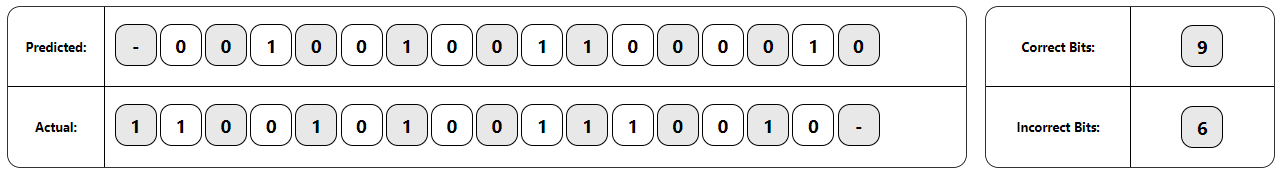
\includegraphics[width=0.9\textwidth]{images/sequence_input.png}
    \caption{Inputted Sequence Displayed in the Web Application}
\end{figure}

This is because that short of a time horizon—10 time steps—would be insufficient to allow the Aggregating Algorithm to identify patterns in the user's inputs and determine which experts should have higher weighting, resulting in poorer predictions by the Learner. However, while there is this distinction in how the sequences are treated, how they are fed back to the user follows \cite{nickerson:2009} in that the concatenated sequence is chunked into groups of 10 when applicable and shown to the user in a separate table (shown in Figure 4). This is because, as discussed in Chapter~\ref{production_of_random_binary_sequences}, the human short-term memory roughly spans 7 (+/- 2) items and by chunking subsequences, the subject can quickly see what they have previously input beyond that span and continue to type inputs that they feel are random.

\begin{figure}[h]
\centering
    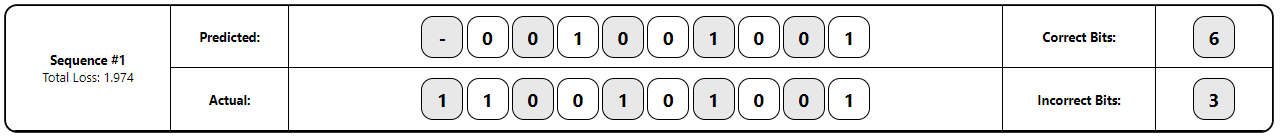
\includegraphics[width=0.9\textwidth]{images/past_sequences.png}
    \caption{Past Sequences Displayed in the Web Application.}
\end{figure}

Given this foundation, we can now discuss how the Aggregating Algorithm for Specialist Experts (AASE) was applied to this experiment. As hinted at in Chapter 2, the primary focus of this dissertation is the Discrete Binary Game defined as $\langle \Gamma, \Omega, \lambda \rangle$ where $\Gamma = [0, 1]$, $\Omega = \{ 0, 1 \}$, and $\lambda = \lambda_{\text{SQ}}(\gamma_t, \omega_t) = (\gamma_t - \omega_t)^2$.

\subsection{Procedure}
Testing
\newpage
\newpage

\section{Analysis of Perceived Randomness}\label{section:Analysis_of_Perceived_Randomness}
\textbf{Data Presentation:} Presentation of collected data in an organised manner.\newline
\textbf{Analytical Techniques:} Methods used to analyse the data.\newline
\textbf{Results:} Detailed presentation of findings.\newline
\textbf{Discussion:} Interpretation of results in the context of perceived randomness.\newline
\textbf{Comparison with Literature:} How the findings align or differ from existing research.\newline
\newpage

\section{Conclusion}\label{section:conclusion}
\subsection{Summary of Findings}\label{subsection:summary_of_findings}
This study aimed to use the Aggregating Algorithm for Specialist Experts to provide a novel insight into the well-documented understanding that humans have difficulty in producing truly random sequences due to cognitive biases and subconscious patterns.

The chi-square tests detailed in Section~\ref{subsection:chi-square_goodness-of-fit} consistently rejected the null hypothesis that humans are good randomisers, indicating deviations from objective randomness in line with previous research~\cite{nickerson:2009}. The plots of difference further confirmed this, achieving a prediction accuracy of 69.19\% on average and implying predictability. This was reflected in the plots consistently below the x-axis, where an individual Expert's predictions were consistently more accurate than the Learner's.

While the individual data deviated from what was expected of true randomness, when the participants' data was aggregated, it showed qualitative similarities. While these similarities do not equate to true randomness, the aggregate tended towards the distribution of a random process, confirming that by aggregating data, the effects of individual biases become increasingly smaller. Ultimately, these results align with the Cognitive Psychology literature, reinforcing the idea that humans struggle to produce truly random outputs, and contribute to the body of research illustrating that human-generated sequences are often more predictable than expected, despite a conscious effort to be random.

\subsection{Limitations}\label{subsection:limitations}
While this study's findings are significant, certain limitations must be acknowledged and addressed in future research.

The first limitation relates to computational power; The AASE implementation was restricted to analysing prefixes up to length 4 as a compromise between computational efficiency and predictive performance. However, considering longer prefixes\textemdash{}extending to the limits of short-term memory\textemdash{}could uncover more intricate and nuanced patterns in human-generated sequences that were previously undetectable.

A second limitation is the small sample size. With only seven participants, individual data heavily influenced the overall results, which limits the study's generalisability. A larger, more diverse sample would minimise this effect and offer a broader evaluation of human randomisation behaviour.

Additionally, future work could extend the Game to consider a \textit{prediction} and \textit{outcome space} that encompasses the entire alphabet, rather than just binary sequences. This would allow the exploration of more complex randomisation tasks, such as the ability to generate random passwords. This could have significant implications for cybersecurity, exposing the weaknesses of human-generated randomness in contexts where security is essential.

\subsection{How to Use the Project}\label{subsection:how_to_use_the_project}
As mentioned in Subsection~\ref{subsection:procedure}, the application is hosted on GitHub Pages, however, it can be run locally from \verb|./aggregating_algorithm/| with:
\begin{center}
    \verb|npm run start|
\end{center}

To use the project, navigate to the website and follow the instructions provided on-screen to conduct the experiment. Once the experiment has concluded, the JSON will be available to download and stored within the directory \verb|./aggregating_algorithm/results/data|. Once moved, one can run the Python script for generating the plots shown in this report by executing the following command from \verb|./aggregating_algorithm/results/|:

\begin{center}
    \verb|python3 generate_plots.py|
\end{center}

\subsection{Self-Assessment}\label{subsection:self-assessment}
This dissertation has been an incredible journey and I am incredibly proud of the result. Not only has it deepened my understanding of the Aggregating Algorithm, but it has also taught me how to manage a personal project. Overall, I can confidently say that the project was a success, both in achieving the objectives outlined in Chapter~\ref{section:introduction} and in preparing for my career. 

This is not to say that the project was not without its challenges. While I was familiar with Python, developing a web application with React.js was a new experience and required more time to learn than originally anticipated which caused delays in my project's timeline that could have been avoided with more cautious planning.

Despite this, the experience has significantly boosted my confidence as a future Machine Learning Engineer. I have learned the value of setting realistic deadlines, how to effectively use online resources, and how to stay current with research\textemdash{}all invaluable skills in the future. Looking ahead, I plan to explore the \textbf{Mixture of Experts (MoE)} ensemble technique as it is conceptually similar to Prediction with Expert Advice, with applications in neural networks which are extremely relevant currently.
\newpage

\bibliographystyle{ieeetr}
\bibliography{bibliography}
\end{document}
